\section{Tudásellenőrző kvíz generálása ismeretlen szavakból}

A funkció célja, hogy egy film végignézése után a felhasználó játékos módon ellenőrizni tudja, hogy az általa ismeretlen szavak mennyire rögzültek filmnézés alatt.
Erre egy kvíz tökéletes megoldás, hiszen így gyorsan, könnyedén, alternatívák közül választva érhet el a felhasználó egy adott pontszámot, amely a filmnézés közben szerzett nyelvtudását tükrözi. Egy ilyen tudásellenőrző még jobban ösztönözheti kitöltőjét az ismeretlen szavak elsajátítására, hiszen a kvízben elért magas pontszám sikerélménnyel párosulhat.

\begin{figure}[h!]
  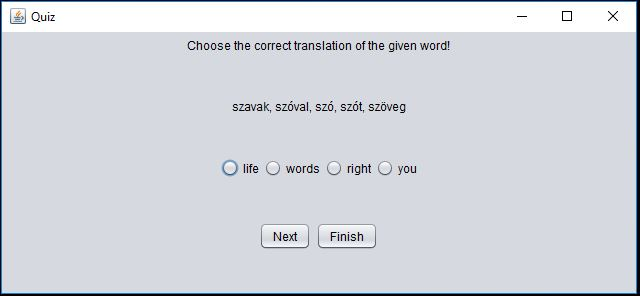
\includegraphics[width=\linewidth]{images/quiz.jpg}
  \caption{Egy a kvízben előforduló kérdés}
  \label{fig:quiz}
\end{figure}

Implementálás során egy \textit{Quiz.java} osztályt készítettem, amely a \textit{JFrame} osztály leszármazottja és képes a kvíz előállítására az adatbázisból kapott adatokból, valamint ennek megjelenítésére, kezelőfelület biztosítására. Ezen belül található egy beágyazott osztály, a \textit{RadioQuestion}, amely egy feleletválasztós kérdést reprezentál, őse a \textit{JPanel} osztály. A működési elv egyszerű: a kvíz ablaka mindig egy kérdést jelenít meg, amit helyes válasz esetén cserél, rossz válasz esetén pedig felugró ablakkal jelzi, hogy a megadott válasz helytelen. Egy kérdés mindig tartalmazza az utasítást, alatta a fordítást vagy fordításokat, lentebb pedig a választási lehetőségeket. A panel alján a \textit{Next}, valamint a \textit{Finish} gombok találhatók meg. Az ablak megtekinthető a \ref{fig:quiz}-es ábrán. A megoldás bejelölése után a \textit{Next}-re kattintva új kérdés következik, a \textit{Finish}-re kattintva pedig befejezhetjük a kvízt, amelyet egy pontösszesítő ablak jelez. A tudásfelmérő elindítható az alkalmazás felső menüsorából, a \textit{Quiz/Take quiz...} menüpontot választva. Ahhoz, hogy a szoftver helyesen tudja megalkotni a kérdéseket alternatívákkal, legalább 6 megfelelő rekordot kell tartalmaznia az adatbázisnak. Amennyiben ez nem teljesül a felhasználót erről egy ablak tájékoztatja, egyébként megjelenik a kvíz ablaka, benne az első kérdéssel.

\begin{spacing}{1.25}
\begin{lstlisting}[caption=Kérdések előállítása, language=java, label={lst:questions}]
words = wordService.getAllByFilename(
   PlayerControlsPanel
   .actualSubtitleFile.getName());

questions = new RadioQuestion[words.size()];
    for (int i = 0; i < questions.length; i++) {
        questions[i] = new RadioQuestion(
            generateRandomAnswers(i),
            words.get(i).getMeaning(),
            words.get(i).getForeignWord(),
            this);
}
\end{lstlisting}
\end{spacing}

  \begin{figure}[h!]
\centering
  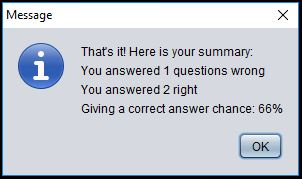
\includegraphics[width=.5\linewidth]{images/summary.jpg}
  \caption{Pontösszesítő ablak}
  \label{fig:summary}
\end{figure}

 A kérdések a \textit{Quiz.java} osztály konstruktorában kerülnek előállításra, és egy tömbben tárolódnak. Először az adatbázisban tárolt szavakat fájlnév szerint lekérdezi, amiket egy listába ment el. Majd ugyanilyen mérettel létrejön egy tömb a kérdés objektumoknak. A függvény végig iterál a tömbön, és minden helyre egy kérdés objektumot hoz létre az alábbi paraméterekkel: Az első paraméter a \textit{generateRandomAnswers} függvény, ami egy \textit{String} tömbbel tér vissza, mely három véletlenszerű alternatívát és egy megoldást tartalmaz. A következő paraméterek az eredeti szó jelentése(i), az eredeti, idegen szó, valamint maga az \textit{Quiz} objektum. A kérdések előállításáért felelős forráskód sorok a \ref{lst:questions}-es kódrészletben találhatók. Az alkalmazás ettől kezdve váltogatja a kérdéseket, amikor pedig mindre válaszoltunk egy összesítő ablakot jelenít meg, amelyben láthatjuk hányszor válaszolunk helyesen, és hányszor helytelenül. Az ablak megtekinthető a \ref{fig:summary}-es ábrán.
 

A bemutatottak alapján megállapítható, hogy a kvíz generálás funkció segíthet rögzíteni, vagy akár elmélyíteni a filmezés közben szerzett információkat, mindezt szórakozással egybekötve.
